\section{Method}
\label{sec:model}

Fig.~\ref{fig:arch} summarises the method. A sensor node at a remote river site records four parameters. At the end of each day it builds a record of the day, adds witnesses, packs both into messages with erasure-coded redundancy, and sends a fixed number $Q$ of messages through a one-way satellite link. The link delivers each message or loses it, and the node never learns which. The server decodes what arrived and answers, for each criterion, exceeded, not exceeded, or undetermined. This section defines the record (Section~\ref{sec:record}), the certificate language and what it can and cannot decide (Section~\ref{sec:cert}), the witnesses (Section~\ref{sec:witness}), the message frame and receiver (Section~\ref{sec:frame}), and the designs compared (Section~\ref{sec:designs}).


\begin{figure}[t]
\centering
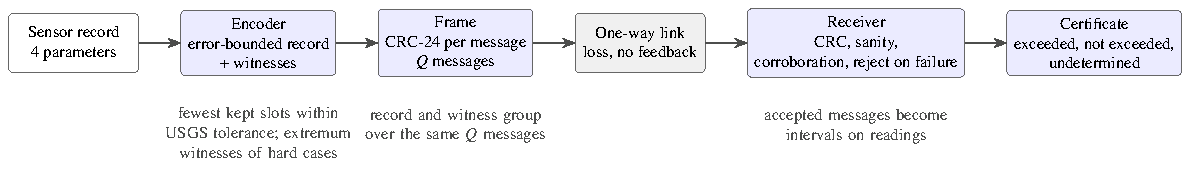
\includegraphics[width=\textwidth]{figs/arch5.pdf}
\caption{Workflow of the method. The node never learns which messages arrived; the receiver uses only accepted messages and the site profile.}
\label{fig:arch}
\end{figure}

\subsection{Record, tolerance, and encoder}
\label{sec:record}
A channel-day is one parameter of one site on one UTC day, with readings $x(t)$, $t = 0, \dots, n-1$, on the parameter's own sampling grid. The tolerance of a reading is $\delta(x) = \max(a, r|x|)$ with the accuracy that the USGS requires of an excellent continuous record \citep{wagner2006}: 0.2\,\textdegree C for temperature; 3\% of the value for specific conductance; the greater of 0.3\,mg/L and 5\% of the value for dissolved oxygen; and 0.2 units for pH. The tolerance is relative to the sensor record; the accuracy of the sensor itself (calibration, fouling, and drift) is outside it.

The encoder selects the fewest kept slots whose piecewise-linear reconstruction keeps every reading within tolerance. This is the minimum-number problem of polygonal approximation \citep{imai1988} with per-reading tolerances, solved exactly by a forward dynamic program over slope windows \citep{orourke1981} in $O(n^2)$ time and $O(n)$ memory per channel-day. Three features make the bound exact and the record self-contained:
\begin{itemize}
  \item Quantisation: every candidate error is computed with the dequantised endpoint values that the server will hold, such that the bound includes quantisation and needs no margin.
  \item Head and tail: the first kept value is held back to midnight and the last is held to the end of the day, such that no value of the previous day is needed.
  \item Censoring: a reading outside the quantiser range is always kept, carried as a flag code, excluded from every bound and decision, and reported as below or above range.
\end{itemize}
A kept reading is a 13-bit code. Linear grids are decimal (0.01\,\textdegree C, 0.005\,mg/L, and 0.002 pH units), and specific conductance uses a logarithmic grid with a step of 0.14\% of the value; the worst quantisation error is 2.5\% of the tolerance.

\subsection{Certificate language}
\label{sec:cert}
The language is independent of the codec: every source of information becomes a closed interval on a reading, and decisions are computed from intervals alone. The server holds, for every reading, an interval $[\mathrm{lo}(t), \mathrm{hi}(t)]$, a set of readings known to be censored, and optional global bounds. The knowledge is valid when every uncensored reading lies in its interval and every global bound holds. Truth statements refer to the sensor record that the loader produced, not to the river.

Sources of information and the intervals they provide:
\begin{itemize}
  \item Base range: the quantiser range of the parameter, valid by the definition of censoring.
  \item Kept value with code $c$: the quantiser cell of $c$, which is far narrower than the tolerance (0 to 0.0025 units for temperature, dissolved oxygen, and pH, and 0.07\% for conductance).
  \item Certified span: the tolerance interval around the reconstruction, valid when the day's bound flag is true and the bounding values of the span arrived. Lemma 1: for $r < 1$ and $x \ge 0$, the set $\{x : |x - \hat{x}| \le \max(a, rx)\}$ is the interval $[\min(\hat{x} - a, \hat{x}/(1 + r)),\ \max(\hat{x} + a, \hat{x}/(1 - r))]$. The two sets whose union defines it share the point $\hat{x}$, such that the union is an interval with the extreme endpoints.
  \item Minimum witness: the cell of the kept extremum value, together with the assertion that every uncensored reading of the day is at least the lower end of that cell; the maximum witness is symmetric.
\end{itemize}
A reading with no information has the base range, such that it blocks a certain no.

Queries have three-valued answers: 1 (certainly yes), 0 (certainly no), or $-1$ (undetermined). Let lo$_\mathrm{eff}(t)$ and hi$_\mathrm{eff}(t)$ be the intervals intersected with the global bounds:
\begin{itemize}
  \item Exceeds below $\theta$ (low dissolved oxygen, low pH): 1 if some hi$_\mathrm{eff}(t) < \theta$; 0 if every lo$_\mathrm{eff}(t) \ge \theta$; otherwise $-1$. The rule for exceeding above $\theta$ is symmetric.
  \item Day minimum and maximum: the minimum lies in $[\min \mathrm{lo}_\mathrm{eff}, \min \mathrm{hi}_\mathrm{eff}]$ and the maximum in $[\max \mathrm{lo}_\mathrm{eff}, \max \mathrm{hi}_\mathrm{eff}]$.
  \item Conductance change: some pair of readings one hour apart with a relative change above 10\%. For readings with intervals $[L_a, U_a]$ and $[L_b, U_b]$, the ratio lies in $[L_b/U_a, U_b/L_a]$ and both ends are attained. A certain no holds when every pair is within 10\% for all values of the intervals. A certain yes holds when no assignment of readings within their intervals keeps every pair within 10\%; for one lag, the pairs form chains, and the set of readings reachable under ``all pairs within 10\%'' is propagated along each chain until it is empty. The pairwise rule ``some single pair is certainly changed'' is sound but incomplete (readings 100, an interval of 100 to 130, and 130 always contain a change, but no pair is certain); therefore, the chain rule is used.
  \item Seven-day mean of daily maxima above 20\,\textdegree C (7DADM): the mean of the seven daily-maximum intervals lies in $[\text{mean of lower ends}, \text{mean of upper ends}]$. A day with no information contributes the base range, never zero and never omission; one missing day therefore blocks a certain no but not a certain yes that the other six days already force.
\end{itemize}

Let $V$ be the uncensored readings of a channel-day (the domain of every query) and $S \supseteq V$ the readings that the server treats as uncensored; a reading in $S \setminus V$ is censored but not known to the server, because it lies inside a certified span and its own code did not arrive. The knowledge is valid on $V$ when every reading in $V$ lies in its interval, every global bound holds on $V$, and every reading that the server holds as censored is censored.

Proposition 1 (soundness): let the knowledge be valid on $V$.
\begin{enumerate}
  \item Every answer 0 of the threshold rules and of the conductance rule, the lower end of every day-minimum interval, and the upper end of every day-maximum interval are correct, whatever $S \setminus V$ is.
  \item Condition B: every reading $t$ in $S \setminus V$ has an interval that reaches the values of genuine readings on both sides, that is, $\mathrm{lo}(t) \le x(u)$ and $\mathrm{hi}(t) \ge x(v)$ for some $u, v$ in $V$. Under condition B, every answer 1 of the threshold rules, both ends of the day-extremum intervals, and every answer of the 7DADM rule are also correct.
  \item Every answer 1 of the conductance rule is correct when no conductance reading of the day is in $S \setminus V$.
\end{enumerate}
Lemma 2 (when condition B holds): a reading in $S \setminus V$ whose certified span is bounded by kept values with uncensored codes satisfies condition B, because its reconstruction lies between the dequantised bounding values, each within half a quantiser step of its true reading, and the half-width of the tolerance interval exceeds half a step for every parameter. Condition B can fail only when a bounding kept value is itself censored; the reconstruction is then pulled to that edge of the quantiser range, and only the queries on that side (below and minimum at the low edge, above and maximum at the high edge) are affected. The proofs are in the supplement (Note S5). As a check, an exhaustive test over every subset of arrived values on small days, with and without each witness, found no interval that excluded the truth and no wrong answer.

The empirical scope of the conditions was counted after the confirmation (post hoc). In the three cohorts (30,854 analysed days), censored readings occurred on 4 days, all at one 2022 site (05576100) and all small negative dissolved-oxygen values; no conductance reading was censored; therefore, part 3 was never at risk. On those 4 days condition B could fail on the low side; the true answer to every dissolved-oxygen query on them was yes at all three threshold sets, and a low-side failure can only add a spurious yes. No reported decision therefore depended on a case that Proposition 1 does not cover.

Proposition 2 (exactness without witnesses, and its failure with them): for the threshold queries and the day extrema, when no witness has arrived, the rule returns an answer other than $-1$ exactly when the query has the same value on all records consistent with the knowledge. With a witness, the rules are sound but not exact. Counterexample: reading 1 in $[3, 10]$, reading 2 in $[4.5, 4.6]$, and a minimum-witness cell $[4.0, 4.01]$. Reading 2 cannot be the minimum; therefore, reading 1 lies in $[4.0, 4.01]$ and ``some reading above 5'' is certainly false, but the box rule returns $-1$. The decisions reported in this study are therefore a lower bound on what the witnesses could decide.

Proposition 3 (identifiability limit): if two records consistent with the received bytes have different answers to a query, no sound decoder can decide that query from those bytes. The tolerance makes this concrete. From a certified span alone, a threshold $\theta$ is decidable at a reading only when the reconstruction is farther from $\theta$ than the half-width of the interval (0.2 pH units, 0.2\,\textdegree C, 3\% of conductance, and the greater of 0.3\,mg/L and 5\% for dissolved oxygen). A reading closer to the threshold can be decided only if its value is carried, because the cell of a kept value is orders of magnitude narrower. This is the formal reason why a record within tolerance misses near-threshold events, and why bytes belong near the threshold and not everywhere. Fig.~\ref{fig:intervals} illustrates the point with constructed values.

\begin{figure}[t]
\centering
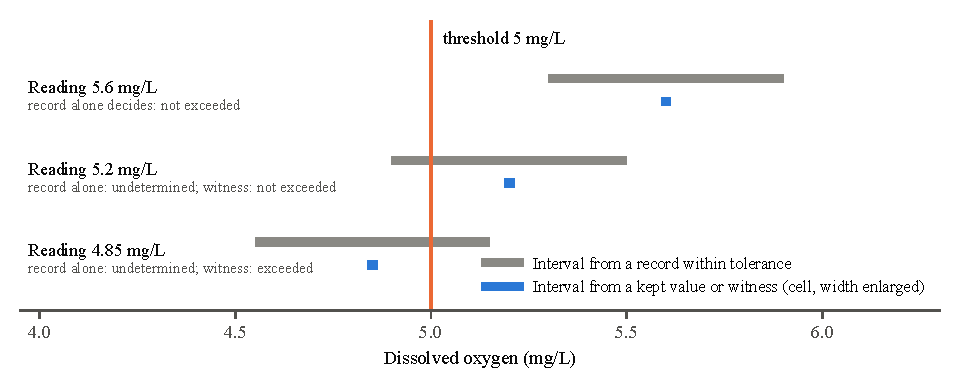
\includegraphics[width=0.85\textwidth]{figs/intervals.pdf}
\caption{Constructed illustration (not data) of the identifiability limit for dissolved oxygen against a threshold of 5 mg/L. The tolerance interval of a record (grey) decides a reading far from the threshold but leaves readings near it undetermined; the cell of a kept value or witness (blue, enlarged for visibility) decides them.}
\label{fig:intervals}
\end{figure}


Soundness is conditional, not unconditional. It requires correct and corroborated messages, an honest encoder, a correct site profile, the quantiser range, and, where the rules use it, assumption R: readings are multiples of the site's reporting resolution. In this study the resolution was inferred from the analysed record itself, and the record contains readings that the loader bridged linearly over gaps of at most two readings. A wrong resolution is unsound: a reading of 7.03 with an assumed resolution of 0.1 yields a certain wrong decision for the threshold 7.01. In development, no resolution could be inferred for dissolved oxygen and pH at 15 of 38 sites, where assumption R was therefore off; in the second confirmation a resolution was inferred for at least one of dissolved oxygen, pH, and temperature at 26 of 35 sites (dissolved oxygen 14, pH 23, temperature 11).

\subsection{Witnesses and hard cases}
\label{sec:witness}
A witness is the quantised extremum of one day and one parameter: the minimum of dissolved oxygen, the minimum and maximum of pH, the maximum of temperature (for the 7DADM), and the conductance rate pair, the two kept values that realise the day's largest hourly relative change. A witness costs 13 bits per code. It carries no slot, because no decision rule uses one.

Not every day needs its witnesses. A case is hard when the record alone is likely to leave the decision open:
\begin{itemize}
  \item within 0.6 mg/L of the dissolved-oxygen threshold, within 0.4 pH units of a pH threshold, or in the event state;
  \item a conductance rate of at least 4\% per hour;
  \item a 7DADM trailing mean within 3\,\textdegree C of 20\,\textdegree C, or with unknown history.
\end{itemize}
These bands were fixed on development data (the 7DADM band and the unknown-history rule after a first run fell short), and the confirmation used them unchanged.

\subsection{Message frame and receiver}
\label{sec:frame}
Each message carries the 23-byte user payload of the KIM1 module \citep{kineis2023kim1}; the operator adds the device identifier and the time of reception \citep{kineis2024formats}. Table~\ref{tab:frame} provides the layout of the frame. A three-byte header (version, block day modulo 64, message index, $K$, and two flags) is not erasure-coded. The 20-byte body carries a CRC-24 (polynomial 0x864CFB) over the header and the rest of the body of every transmitted message, whether data or parity, an optional witness section, and one Reed--Solomon symbol of the record units over GF($2^8$). The block day is unwrapped from the operator's reception time.

\begin{table}[t]
\centering
\caption{Message frame (23-byte payload).}
\label{tab:frame}
\small
\begin{tabularx}{\textwidth}{@{}llX@{}}
\toprule
Part & Bits & Content \\
\midrule
Header (not coded) & 24 & version (2); block day modulo 64 (6); message index (7); $K$, the record data units (7); coded flag (1); witness-group flag (1) \\
Check & 24 & CRC-24 over the header and the rest of the body, in every message \\
Witness descriptor (if flagged) & 8 & $k_w$, the data units of the witness group (3); presence mask of the five witness objects (5) \\
Witness symbol (if flagged) & $8 s_w$ & one symbol of the witness group, with $s_w = \lceil \lceil 13 \cdot \text{codes} / k_w \rceil / 8 \rceil$ bytes \\
Record symbol & rest & one Reed--Solomon symbol of the record data units \\
\bottomrule
\end{tabularx}
\end{table}

A record data unit carries up to three segments of kept values and a hosted-witness section: a flag, a 5-bit presence mask, and 13-bit codes in the spare room of the unit. Hosted witnesses cost no record capacity. Without witnesses the 136-bit record symbol holds four record values of 24 bits after 24 bits of unit overhead, which leaves 16 spare bits; a layered witness group takes whole bytes from the record symbol.

The check length was chosen on development data by a rule written before the comparison: four candidate frames (CRC-16 as in the earlier version, CRC-16 with a record-level CRC-32, CRC-24, and both) were compared by the expected number of days with a false certificate per million days at an assumed bit-error rate of $10^{-3}$, with a limit of 0.5, and among the frames that met the limit the one with the highest whole-record recovery, with ties going to the simpler frame, was selected. Only the two CRC-24 frames met the limit, and the simpler one was selected. The CRC-24 costs one record value per message (four instead of five) and lowers the probability that a corrupted message passes the check by a factor of 256.

The receiver applies these rules:
\begin{enumerate}
  \item Accept a message only if its CRC passes, and drop duplicates; an object that is not a message of the right length counts as a failed message.
  \item Decode the record from any $K$ accepted messages and the witness group from any $k_w$ accepted messages; with a check on every message there is no retry over combinations of parity messages.
  \item Sanity: reject values outside the site profile or out of planned order, and censored witness codes.
  \item Corroboration: when more messages arrive than are needed, re-encode the decoded units and compare with every other accepted message; any mismatch rejects the block, and nothing is certified from it. A witness descriptor that differs between messages, or two CRC-valid copies of one message that disagree, also reject the block.
  \item Any failure while decoding a block, of whatever kind, rejects the record and the witnesses of that block.
  \item Produce certificates by the rules above from accepted, corroborated content only. A day on which no reading is uncensored has no defined extremum, and its extremum interval is unbounded, which leaves every decision that needs it undetermined.
\end{enumerate}
A limit remains: a record value with a censored code (the lowest or highest code) passes the sanity rule, because honest records carry such codes for readings outside the quantiser range, and it removes that reading from every decision. Section~\ref{sec:integrity} reports how often a forged message led to a wrong decision.

\subsection{Designs compared}
\label{sec:designs}
The confirmation compared three designs on the same loss draws at byte level: real messages were built, lost, decoded by the receiver, and the decisions were made from the decoded values and witness codes only.
\begin{itemize}
  \item Record only: the record, with $D_1$ data units and $Q - D_1$ parity messages of a systematic Reed--Solomon code, such that any $D_1$ messages recover it.
  \item 3b rule: the generalised rule of this study. Witnesses of hard cases form a layered group in their own protected message columns ($k_w \le 2$); witnesses of easy cases are hosted in the spare room of the last record unit. In the language of priority encoding transmission \citep{albanese1996}, the record and the witness group are two priority levels over the same $Q$ messages.
  \item Flags plus record: the record-only blocks plus the answers to the four configured queries (4 bits) in every message. The flag field fits in the 16 spare bits of the record symbol; therefore, the record is the same as in the record-only design. The server takes the certificate decision when it is certain and otherwise the configured answer whenever any message arrived; an unconfigured threshold is decided by the record or by monotone implication from the configured answer. The flag answers are taken from the true record; therefore, this comparator is idealised; it is the fair comparator for the witness design because it uses everything a flag node would receive.
\end{itemize}
In development, the following were also compared in an abstract slot model (a message holds a whole number of value slots, a group is a systematic maximum-distance-separable code, and witnesses occupy whole slots): decision flags that do not use the record, an exact allocator of witnesses to columns, two hybrids of flags and witnesses, the same layering on random days (a control for targeting), send-on-delta with hold reconstruction \citep{diazcacho2017sod}, and the record at half the tolerance. These were not re-run in the final version of the method, and no claim rests on them (Section~\ref{sec:devres}). The slot model was also run in the confirmation as a cross-check of the byte-level results; it assigns the witness group whole slots and therefore overstates the record cost of the 3b rule.
